\documentclass[]{article}
\newcommand{\FileDepth}{../..}
\input{\FileDepth/Formats/AssignmentBasics.tex}
\usepackage{cancel}%This is special for Activities 4 and 5.
%opening
\newcommand{\SecType}{X}
\newcommand{\Week}{X}
\title{Interactions and the Third Law}
\author{Benjamin Bauml}
\date{Spring 2024}
\pagestyle{fancy}
\rhead{PH 221}
\chead{Spring 2024}
\lhead{Week \Week}

% For Assignment, leave Purpose as 1. For Worksheet, set to 2. For Student Solution, set to 3. For Teacher Solution, set to 4.
% If you want keep the pieces from being called manually, set DefOnly to 0.
\newcommand{\Purpose}{4}
\newcommand{\DefOnly}{1}

% Version 2024-04-27
% Changes
% 2024-02-21 Added xstring package to enable smooth implementation of new \ModePage command.
% 2024-04-27 Set up to split activities and formatting aspects into separate files. Removed dependence on xcomment. Added an automatic counter to number the activities in a problem set.
\usepackage{tcolorbox}
\usepackage{xstring}
% You will want the following four lines in your document (the last two uncommented):
% For Assignment, leave Purpose as 1. For Worksheet, set to 2. For Student Solution, set to 3. For Teacher Solution, set to 4.
% If you want keep the pieces from being called manually, set DefOnly to 0.
%\newcommand{\Purpose}{4}
%\newcommand{\DefOnly}{1}
\newcommand{\Exclusion}{0}
\newcommand{\PageTurn}{0}
\newcommand{\GrayProb}{0}
\newcommand{\Tipsy}{0}

% Assignment
\if\Purpose1
\renewcommand{\Exclusion}{1}
\fi
% Worksheet
\if\Purpose2
\renewcommand{\Exclusion}{1}
\renewcommand{\PageTurn}{1}
\fi
% Student Solution
\if\Purpose3
\renewcommand{\PageTurn}{1}
\renewcommand{\GrayProb}{1}
\fi
% Teaching Copy
\if\Purpose4
\renewcommand{\PageTurn}{1}
\renewcommand{\GrayProb}{1}
\renewcommand{\Tipsy}{1}
\fi

\def \NewQ {0}
\def \PForce {0}
\newcommand{\MaybePage}[1]{
	\def \PForce {#1}
	\if\PForce1
	\newpage
	\else
	\if\NewQ0
	\gdef \NewQ {\PageTurn}
	\else
	\newpage
	\fi
	\fi
}

\newcommand{\ModePage}[1]{
	\IfSubStr{#1}{\Purpose}{\newpage}{}
}

\newcounter{ActNumber}
\setcounter{ActNumber}{0}

\newcommand{\Problem}[4][0]{%The first argument is optional, and if it is set to 1, the \newpage will be forced. The second argument is the name of the activity, the third is the command the activity is stored as, and the fourth is the actual problem statement.
\newcommand{#3}{
\MaybePage{#1}
\addtocounter{ActNumber}{1}
\section*{\SecType\Week-\theActNumber: #2}
\if\GrayProb1
\begin{tcolorbox}[colback=lightgray,colframe=lightgray,sharp corners,boxsep=1pt,left=0pt,right=0pt,top=0pt,bottom=0pt,after skip=2pt]
\else
\begin{tcolorbox}[colback=white,colframe=white,sharp corners,boxsep=1pt,left=0pt,right=0pt,top=0pt,bottom=0pt,after skip=2pt]
\fi
#4
\end{tcolorbox}\noindent
}
\if\DefOnly0
\else
#3
\fi
}
	
\newcommand{\ProblemSub}[3][0]{%The first argument is optional, and if a string of numbers is entered into it, it will force a \newpage in any \Purpose that shows up in the string. For example, "13" would lead to the newpage being forced in modes 1 and 3. The second is the command the activity is stored as, and the third is the actual problem statement.
\newcommand{#2}{
\ModePage{#1}
\if\GrayProb1
\begin{tcolorbox}[colback=lightgray,colframe=lightgray,sharp corners,boxsep=1pt,left=0pt,right=0pt,top=0pt,bottom=0pt,after skip=2pt]
\else
\begin{tcolorbox}[colback=white,colframe=white,sharp corners,boxsep=1pt,left=0pt,right=0pt,top=0pt,bottom=0pt,after skip=2pt]
\fi
#3
\end{tcolorbox}\noindent
}
\if\DefOnly0
\else
#2
\fi
}
		
\newcommand{\Solution}[2]{%The first argument is the command the solution is stored as, and the second is the actual solution.
\newcommand{#1}{
\if\Exclusion0
#2
\fi
}
\if\DefOnly0
\else
#1
\fi
}
		
\newcommand{\ProblemFig}[2]{%The first argument is the command the figure is stored as, and the second is the actual figure.
\newcommand{#1}{
\begin{figure}[h]
#2
\end{figure}
}
\if\DefOnly0
\else
#1
\fi
}
		
\newcommand{\TeachingTips}[1]{
\if\Tipsy1
\begin{tcolorbox}[colback=lightgray,colframe=black]
#1
\end{tcolorbox}
\fi
}

\newcommand{\FBDaxes}[4][2]{
	\begin{scope}[shift={(#2)},rotate=#3]
		% x-axis
		\draw[thick,->] (-#1,0) -- (#1,0);
		\node[anchor=west] at (#1,0) {$x$};
		% y-axis
		\draw[thick,->] (0,-#1) -- (0,#1);
		\node[anchor=south] at (0,#1) {$y$};
		\coordinate (#4) at (0,0);
	\end{scope}
}
\newcommand{\FBDvectorMA}[4]{
	\begin{scope}[shift={(#1)}]
		\coordinate (#4tip) at ({#2*cos(#3)},{#2*sin(#3)});
		\draw[ultra thick,blue,->] (#1) -- (#4tip);
	\end{scope}
}
\newcommand{\FBDvectorXY}[3]{
	\begin{scope}[shift={(#1)}]
		\coordinate (#3tip) at (#2);
		\draw[ultra thick,blue,->] (0,0) -- (#3tip);
	\end{scope}
}
\newcommand{\FBDdot}[1]{
	\filldraw[black] (#1) circle (3pt);
}
\newcommand{\FBDbox}[5][1]{
	\begin{scope}[shift={(#2)},rotate=#3]
		\filldraw[color=black,fill=white,thick] ({-#1/2},{#1/2}) -- ({-#1/2},{-#1/2}) -- ({#1/2},{-#1/2}) -- ({#1/2},{#1/2}) -- cycle;
		% Left side coordinates
		\coordinate (#4ltq) at ({-#1/2},{#1/4});
		\coordinate (#4lcent) at ({-#1/2},0);
		\coordinate (#4lbq) at ({-#1/2},{-#1/4});
		% right side coordinates
		\coordinate (#4rtq) at ({#1/2},{#1/4});
		\coordinate (#4rcent) at ({#1/2},0);
		\coordinate (#4rbq) at ({#1/2},{-#1/4});
		% top coordinates
		\coordinate (#4tlq) at ({-#1/4},{#1/2});
		\coordinate (#4tcent) at (0,{#1/2});
		\coordinate (#4trq) at ({#1/4},{#1/2});
		% bottom coordinates
		\coordinate (#4blq) at ({-#1/4},{-#1/2});
		\coordinate (#4bcent) at (0,{-#1/2});
		\coordinate (#4brq) at ({#1/4},{-#1/2});
		% corners
		\coordinate (#4tl) at ({-#1/2},{#1/2});
		\coordinate (#4tr) at ({#1/2},{#1/2});
		\coordinate (#4bl) at ({-#1/2},{-#1/2});
		\coordinate (#4br) at ({#1/2},{-#1/2});
		\node at (0,0) {#5};
	\end{scope}
}

\begin{document}
\maketitle
\begin{center}
	This material is borrowed/adapted from Chapter 7 of the \textit{Student Workbook} for \textit{Physics for Scientists and Engineers}.
\end{center}

\Problem{Interactions and the Third Law}{\InterandThird}{
For the following situations, draw free-body diagrams and indicate the Newton’s third law pairs.
}
\ProblemSub{\InterandThirdA}{
(a) A massless string pulls a box across the floor. Friction is not negligible.
}
\Solution{\InterandThirdASol}{
\begin{figure}[h]
	\centering
	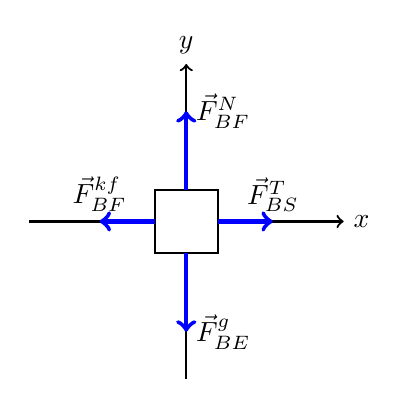
\begin{tikzpicture}
		\FBDaxes{0,0}{0}{axes}
		%This is just to test the FBDbox command.
		%\FBDbox{2,2}{0}{box}{$m$}
		%\draw (boxbr) -- (2,0) -- (boxtr) -- (0,2) -- (boxtl) -- (-2,0) -- (boxbl) -- (0,-2) -- cycle;
		%\draw (boxrbq) -- (2,0) -- (boxrtq) -- (boxtrq) -- (0,2) -- (boxtlq) -- (boxltq) -- (-2,0) -- (boxlbq) -- (boxblq) -- (0,-2) -- (boxbrq) -- cycle;
		%\draw (2,0) -- (boxrcent);
		%\draw (-2,0) -- (boxlcent);
		%\draw (0,2) -- (boxtcent);
		%\draw (0,-2) -- (boxbcent);
		\FBDbox[0.8]{axes}{0}{box}{}
		\FBDvectorXY{boxrcent}{0.7,0}{FT}
		\node[anchor=south] at (FTtip) {$\vec{F}^{T}_{BS}$};
		\FBDvectorXY{boxlcent}{-0.7,0}{FK}
		\node[anchor=south] at (FKtip) {$\vec{F}^{kf}_{BF}$};
		\FBDvectorXY{boxtcent}{0,1}{FN}
		\node[anchor=west] at (FNtip) {$\vec{F}^{N}_{BF}$};
		\FBDvectorXY{boxbcent}{0,-1}{FG}
		\node[anchor=west] at (FGtip) {$\vec{F}^{g}_{BE}$};
	\end{tikzpicture}
\end{figure}

There are no 3rd law pairs in my above representation, as I only drew one free-body diagram. Technically, each of these forces is part of a 3rd law pair ($\vec{F}^{N}_{BF}$ with $\vec{F}^{N}_{FB}$, $\vec{F}^{kf}_{BF}$ with $\vec{F}^{kf}_{FB}$, $\vec{F}^{T}_{BS}$ with $\vec{F}^{T}_{SB}$, and $\vec{F}^{g}_{BE}$ with $\vec{F}^{g}_{EB}$), but since I didn't draw free-body diagrams for the floor, the string, or the Earth, the other vector of each pair is not present.

We know that the normal and gravitational forces are balanced on this box, though we don't know if the force of tension is balanced against the force of kinetic friction. I drew them equal for simplicity, but if we had more information about the box's acceleration, we might want to redraw them with different lengths.
}
\ProblemSub[34]{\InterandThirdB}{
(b) The bottom block is pulled by a massless string. Friction is not negligible. Treat the two blocks as separate objects.
}
\ProblemFig{\InterandThirdBFig}{
\centering
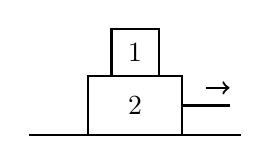
\begin{tikzpicture}
	\begin{scope}[scale=1.5]
	\draw[thick] (0,0) rectangle (0.8,0.5);
	\node at (0.4,0.25) {2};
	\draw[thick] (0.2,0.5) rectangle (0.6,0.9);
	\node at (0.4,0.7) {1};
	\draw[thick] (0.8,0.25) -- (1.2,0.25);
	\draw[thick] (-0.5,0) -- (1.3,0);
	\draw[thick,->] (1,0.4) -- (1.2,0.4);
	\end{scope}
\end{tikzpicture}
}
\Solution{\InterandThirdBSol}{

If the blocks are speeding up, then I would draw the following diagrams:

\begin{figure}[h]
	\centering
	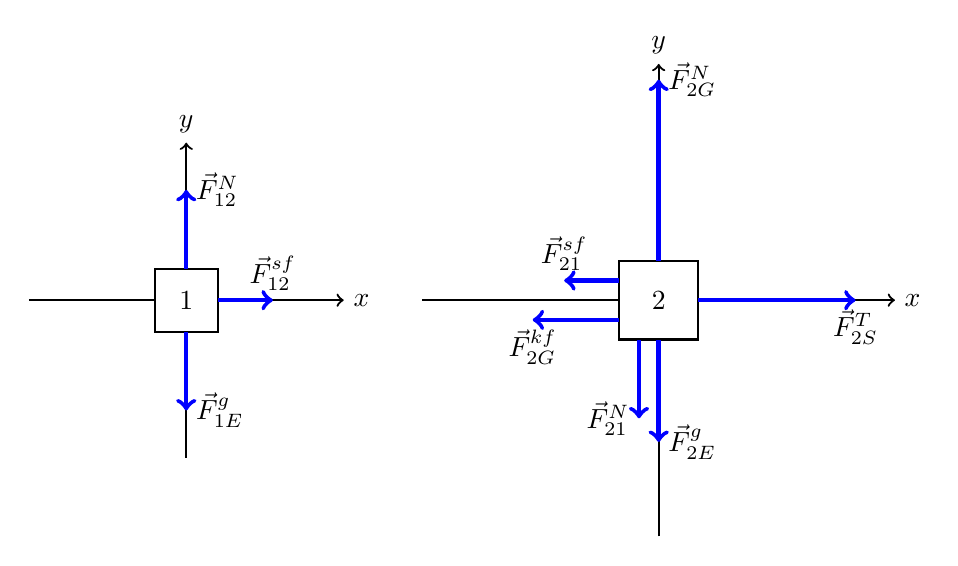
\begin{tikzpicture}
		\FBDaxes{-3,0}{0}{taxes}
		\FBDbox[0.8]{taxes}{0}{tbox}{1}
		\FBDvectorXY{tboxrcent}{0.7,0}{FS12}
		\node[anchor=south] at (FS12tip) {$\vec{F}^{sf}_{12}$};
		\FBDvectorXY{tboxtcent}{0,1}{FN12}
		\node[anchor=west] at (FN12tip) {$\vec{F}^{N}_{12}$};
		\FBDvectorXY{tboxbcent}{0,-1}{FG1}
		\node[anchor=west] at (FG1tip) {$\vec{F}^{g}_{1E}$};
		\FBDaxes[3]{3,0}{0}{baxes}
		\FBDbox{baxes}{0}{bbox}{2}
		\FBDvectorXY{bboxltq}{-0.7,0}{FS21}
		\node[anchor=south] at (FS21tip) {$\vec{F}^{sf}_{21}$};
		\FBDvectorXY{bboxblq}{0,-1}{FN21}
		\node[anchor=east] at (FN21tip) {$\vec{F}^{N}_{21}$};
		\FBDvectorXY{bboxlbq}{-1.1,0}{FK}
		\node[anchor=north] at (FKtip) {$\vec{F}^{kf}_{2G}$};
		\FBDvectorXY{bboxrcent}{2,0}{FT}
		\node[anchor=north] at (FTtip) {$\vec{F}^{T}_{2S}$};
		\FBDvectorXY{bboxbcent}{0,-1.3}{FG2}
		\node[anchor=west] at (FG2tip) {$\vec{F}^{g}_{2E}$};
		\FBDvectorXY{bboxtcent}{0,2.3}{FN2}
		\node[anchor=west] at (FN2tip) {$\vec{F}^{N}_{2G}$};
	\end{tikzpicture}
\end{figure}

We can see that the static friction from block 2 pulls block 1 to the right, and therefore the static friction from block 1 pulls block 2 in the opposite direction, working against its motion.

On the other hand, if the blocks are slowing down, I would instead draw the following diagrams:

\begin{figure}[h]
	\centering
	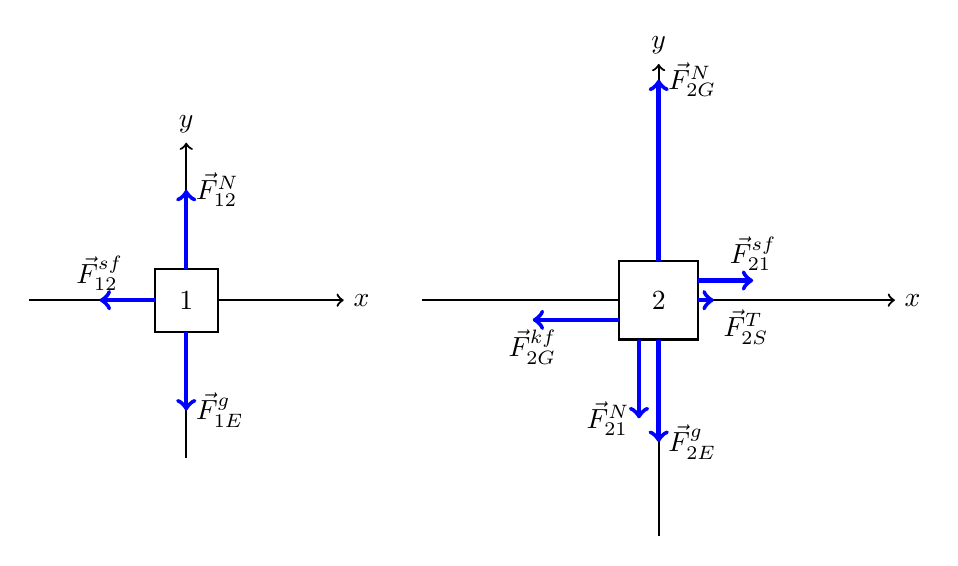
\begin{tikzpicture}
		\FBDaxes{-3,0}{0}{taxes}
		\FBDbox[0.8]{taxes}{0}{tbox}{1}
		\FBDvectorXY{tboxlcent}{-0.7,0}{FS12}
		\node[anchor=south] at (FS12tip) {$\vec{F}^{sf}_{12}$};
		\FBDvectorXY{tboxtcent}{0,1}{FN12}
		\node[anchor=west] at (FN12tip) {$\vec{F}^{N}_{12}$};
		\FBDvectorXY{tboxbcent}{0,-1}{FG1}
		\node[anchor=west] at (FG1tip) {$\vec{F}^{g}_{1E}$};
		\FBDaxes[3]{3,0}{0}{baxes}
		\FBDbox{baxes}{0}{bbox}{2}
		\FBDvectorXY{bboxrtq}{0.7,0}{FS21}
		\node[anchor=south] at (FS21tip) {$\vec{F}^{sf}_{21}$};
		\FBDvectorXY{bboxblq}{0,-1}{FN21}
		\node[anchor=east] at (FN21tip) {$\vec{F}^{N}_{21}$};
		\FBDvectorXY{bboxlbq}{-1.1,0}{FK}
		\node[anchor=north] at (FKtip) {$\vec{F}^{kf}_{2G}$};
		\FBDvectorXY{bboxrcent}{0.2,0}{FT}
		\node[anchor=north west] at (FTtip) {$\vec{F}^{T}_{2S}$};
		\FBDvectorXY{bboxbcent}{0,-1.3}{FG2}
		\node[anchor=west] at (FG2tip) {$\vec{F}^{g}_{2E}$};
		\FBDvectorXY{bboxtcent}{0,2.3}{FN2}
		\node[anchor=west] at (FN2tip) {$\vec{F}^{N}_{2G}$};
	\end{tikzpicture}
\end{figure}

We can see here that the static friction on 1 by 2 must act to slow down block 1, but the static friction on 2 by 1 points in the same direction as the motion---in a sense, the bottom block can feel the top block trying to keep going forward at its original speed.

The third law pairs here are the static frictions, $\vec{F}^{sf}_{12}$ and $\vec{F}^{sf}_{21}$, and the normal forces between the blocks, $\vec{F}^{N}_{12}$ and $\vec{F}^{N}_{21}$.
}
\ProblemSub[34]{\InterandThirdC}{
(c) A skateboarder is pushing on the ground to speed up. Treat the person and the skateboard as separate objects.
}
\Solution{\InterandThirdCSol}{The person has one foot on the board (so there will be a normal and a frictional force from that) and one foot on the ground (so there will be a normal and a frictional force from that). With the long range force of gravity, that makes five forces total on the person.

The board is touching the person (so there will be a normal and a frictional force from that) and the ground (so there will be a normal and a frictional force from that). With the long range force of gravity, that makes five forces total on the skateboard as well.

\begin{figure}[h]
	\centering
	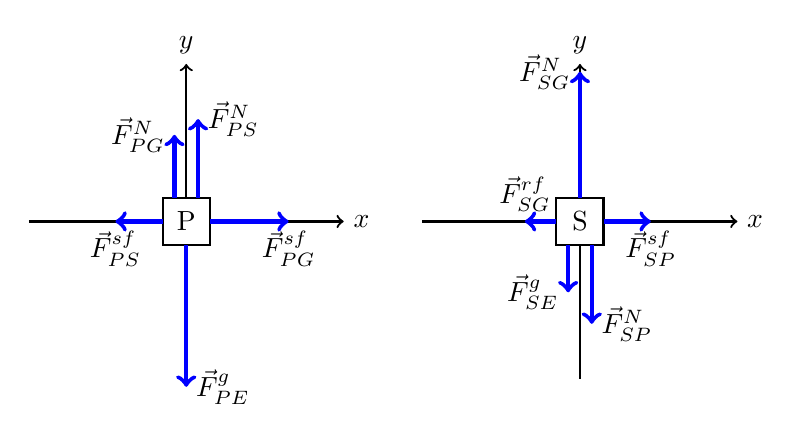
\begin{tikzpicture}
		\FBDaxes{-2.5,0}{0}{paxes}
		\FBDbox[0.6]{paxes}{0}{pbox}{P}
		\FBDvectorXY{pboxtrq}{0,1}{FNPS}
		\node[anchor=west] at (FNPStip) {$\vec{F}^{N}_{PS}$};
		\FBDvectorXY{pboxtlq}{0,0.8}{FNPG}
		\node[anchor=east] at (FNPGtip) {$\vec{F}^{N}_{PG}$};
		\FBDvectorXY{pboxbcent}{0,-1.8}{FGP}
		\node[anchor=west] at (FGPtip) {$\vec{F}^{g}_{PE}$};
		\FBDvectorXY{pboxlcent}{-0.6,0}{FSPS}
		\node[anchor=north] at (FSPStip) {$\vec{F}^{sf}_{PS}$};
		\FBDvectorXY{pboxrcent}{1,0}{FSPG}
		\node[anchor=north] at (FSPGtip) {$\vec{F}^{sf}_{PG}$};
		\FBDaxes{2.5,0}{0}{saxes}
		\FBDbox[0.6]{saxes}{0}{sbox}{S}
		\FBDvectorXY{sboxbrq}{0,-1}{FNSP}
		\node[anchor=west] at (FNSPtip) {$\vec{F}^{N}_{SP}$};
		\FBDvectorXY{sboxtcent}{0,1.6}{FNSG}
		\node[anchor=east] at (FNSGtip) {$\vec{F}^{N}_{SG}$};
		\FBDvectorXY{sboxblq}{0,-0.6}{FGS}
		\node[anchor=east] at (FGStip) {$\vec{F}^{g}_{SE}$};
		\FBDvectorXY{sboxrcent}{0.6,0}{FSSP}
		\node[anchor=north] at (FSSPtip) {$\vec{F}^{sf}_{SP}$};
		\FBDvectorXY{sboxlcent}{-0.4,0}{FRSG}
		\node[anchor=south] at (FRSGtip) {$\vec{F}^{rf}_{SG}$};
	\end{tikzpicture}
\end{figure}

In drawing these, I assumed that the person and skateboard are speeding up to the right. As such, the person is pushing backward (to the left) against the ground with their foot, which means the static friction from the ground must point right to keep the foot from slipping backward. As such, this static friction is what propels the person forward (to the right). Similarly, the static friction on the board by the person's other foot also propels the skateboard forward with the skateboarder. Conversely, the static friction on the skateboarder by the skateboard points to the left; the person feels dragged backward a bit as the skateboard's inertia resists being dragged along with them.

The third law pairs are the forces of static friction between the person and the skateboard ($\vec{F}^{sf}_{PS}$ and $\vec{F}^{sf}_{SP}$) and the normal forces between the person and the skateboard ($\vec{F}^{N}_{PS}$ and $\vec{F}^{N}_{SP}$).

As a side note, you may notice that I labeled the friction between the skateboard and the ground as $\vec{F}^{rf}_{SG}$. We don't teach this in the course, but $rf$ is meant to stand for a third friction model: \textit{rolling friction}. The important thing is, we cannot call this friction between the board and the ground kinetic. Kinetic friction is only for things sliding against each other, and here, the wheels do not slip against the ground. Since the wheels are not slipping, you could think of there being a force of static friction that keeps the wheels from slipping (they would be sliding to the right if there were no friction, so this static friction would still point left in this case, where the wheels are not propelling the skateboard---unlike an FBD for a car). However, rolling friction is more accurate, as it captures the additional interactions inherent in a surface sinking into and lifting off from another surface as it rolls across.
}
\end{document}